%Template file for MATH96012 project 4 discussion and figures
\documentclass{article}
\usepackage[utf8]{inputenc}
\title{MATH96012 Project 4}

\author{Alexander John Pinches CID: 01201653}

\usepackage{graphicx}

\begin{document}

\maketitle



%---------------- Part 1 -------------------
\section*{Question 1.1}
As A is a very sparce matrix with its sparcity increasing as n increases 
creating A as a dense matrix will use lots of memory and be slower for
the matrix multiplication as there will be lots of multiplying by zero
so instead we store the values and their row and column index this uses
less memory for n large and is more efficent when performing the multiplication.
Also switching the row and column index allows us to easily multiply by A transposed. 

We then only need to perform the multiplication for the values in the sparce form of A
with their location in the product determined by their row index.

\section*{Question 1.4}
The time taken for each method is shown in figure \ref{fig1}. We see that the
python implimentation is by far the slowest especially for large N with a large jump
at 2000. The F90 jacobian implimentation is slower than the SGI OpenMP implimentation
this will be due to the parallelisation which becomes more significant the larger N is.
So we should always use the SGI fortran implementation for the fastest results.
 \newpage

\subsection*{Figures}
\begin{figure}[h!]
\centering
%Uncomment line below to display figure saved as fig1.png
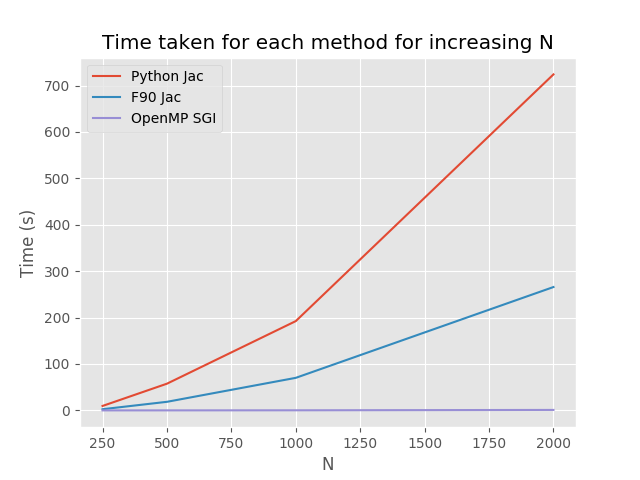
\includegraphics[width=0.6\textwidth]{time.png}
\caption{Time taken for increasing N}
\label{fig1}
\end{figure}

%Add further figures as needed here
\newpage

\section*{Question 1.5}
We can use the MPE\_DECOMP1D subroutine from Argonne National Laboratory to 
give the start and end index for each process. We can then have each process
calculate its portion of Md it will need the start to end columns and rows of A for the multiplication by A and then we can calculate the get the scalars for
$e^{T}e$ and $d^{T}Md$ for its start and end we then divide these two numbers.
To get K we then sum across all processes using MPI\_Allreduce as we want the sum
to be on each process with the operation specified as MPI\_SUM. Using the k
we can then calculate the new x and e for each process between their start and end.
We can then calculate $e^{T}e$ for the new e and get the scalar $\mu$ for each 
process then use MPI\_Allreduce with MPI\_SUM like before. Then each process can 
calculate its new d. We also calculate the max change in x on each process
then use MPI\_Allreduce with MPI\_MAX to see the max change in x across all processes.
Repeating these steps till we reach the max number of iterations
or the change in x falls below the tolerance.

The advantage of the MPI approach is we dont have to rely on shared memory
so we can distribute the work across computers without having to have memory
shared by both. Also, we dont have to wait whilst the process is forked each time 
we want to do something in parallel. This makes it more scalable as we arent limited by cores on
a single machine and we have less memory overhead from having to copy arrays for each core.
However the communication between processes with MPI is much slower as you have to send data 
from one process to another. Whereas in openmp everything is kept locally in memory which 
is quickly acessed by each core especially if its small enough to be kept in the cpus
cache.

%---------------- End Part 1 -------------------


%---------------- Part 2 -------------------
\section*{Question 2.3}
As we know that $max(a_{i}) \le min(nlocal)$ we need to have the $nlocal-1$ 
values above and below the last and first values in ylocal we store these in f. Whose first nlocal-1 values
are from the process below the next nlocal are calculated by the current process and then the 
nlocal -1 after this are calculated by the process above. Which we get 
from the process above and below by them sending their ylocal after each update of ylocal and storing in f. We use MPI\_REDUCE
to collect the sum of $exp(i\theta)$ for each process and store it in process 0. Taking the 
absolute value and dividing by N after the loop on process 0. We use MPI\_GATHER to take ylocal from
each process and put it into y on process 0.


\section*{Question 2.4}
The best approach would be to split the theta space into a grid. The theta
space is a MxM grid and if we have say N processes we want each process to be given
a $\frac{M}{\sqrt{N}}$x$\frac{M}{\sqrt{N}}$ space and to send its results to the processes
above below and to the left and right of itself on this grid. This will mean that
there will need to be 2 more MPI\_ISEND and MPI\_RECV calls to send the extra the ys calculated
by other processes. For a given process with $id=x$ it will need to get 
the results from and give its results to the process above it in the grid with id $mod((FLOOR(\frac{x}{\sqrt{N}})-1)*\sqrt{N}+mod(x,\sqrt{N}),N)$
and below at $mod((FLOOR(\frac{x}{\sqrt{N}})+1)*\sqrt{N}+mod(x,\sqrt{N}),N)$ and the process to its left and right on the grid
at $(FLOOR(\frac{x}{\sqrt{N}}))*\sqrt{N}+mod(x-1,\sqrt{N})$ and $(FLOOR(\frac{x}{\sqrt{N}}))*\sqrt{N}+mod(x+1,\sqrt{N})$.
we dont need the results from other processes because of the restrictions on the maximum
size of a. We would also of course have to change the sumSin and RHS to allow to sum across an additional axis and to change
the dimensions of the arrays to allow for the extra dimension in the 2d case.
%---------------- End Part 2 -------------------




%---------------- End document -------------------


\end{document}
